% ---------------------------------------------------------------------
% Section 6: Hardware validation
% ---------------------------------------------------------------------
\section{Hardware Validation}\label{sec:hardware}

\subsection{Platform, protocol, and experimental matrix}

The platform is a six-degree-of-freedom B601-DM manipulator: joint bus and state feedback at $500\,\mathrm{Hz}$, control period $\Delta t=10\,\mathrm{ms}$, and a torque interface $\boldsymbol\tau=\hat M\ddot{\boldsymbol q}_{\mathrm{ref}}+\hat C\dot{\boldsymbol q}+\hat{\boldsymbol g}$ augmented by feedforward model-completion terms (viscous friction $0.8$, Coulomb friction $[0,\,0.08,\,1.69,\,0,0,0]\,\mathrm{N\,m}$, and rotor inertia $\mathrm{diag}(0.01)$; none of these are feedback). The task is a $10\,\mathrm{s}$ point-to-point min-jerk motion to a fixed target pose ($\max\|\dot{\boldsymbol q}\|=0.253\,\mathrm{rad/s}$, $\max\|\ddot{\boldsymbol q}\|=2.44\,\mathrm{rad/s^2}$). The experimental matrix combines four control laws with DC stiffness levels $k\in\{8,16,24,36\}\,\mathrm{s^{-2}}$ and firmware tether springs $K_{\mathrm{tr}}\in\{12,30,60\}\,\mathrm{N\,m/rad}$, where the four laws are: C1 (proposed, \eqref{eq:5.2}); C2, the spiral-logarithm second-order baseline of \cite{Ch20}; C3, the first-order $H_\infty$ law of \cite{P2} bridged to acceleration level through a velocity servo with $k_{\mathrm{servo}}=20$; and C4, a classical decoupled SE(3) second-order law with quaternion-vector pose error. The tether spring pulls along the planned reference trajectory (not to a fixed anchor) and is lowered by one order of magnitude from the vendor default of $120/18$ in order to purify the task law. The $k{=}36$ tier was run 22 times (one run per setting enters the figures and tables), and all 33 valid runs produced zero torque saturation, with the acceleration governor active in at most $11.2\%$ of frames.

All laws are balanced according to the transmission factors of the linearization \eqref{eq:5.8} so that both channels share the same DC stiffness $k$ (C1: $p_O{=}4k$, $p_T{=}k$; C2: $K_P{=}kI_6$; C4: $K_{p,O}{=}2k$, $K_{p,T}{=}k$; C3: $k_O{=}\sqrt2/\gamma_O$, $k_T{=}\sqrt2/\gamma_T$ with servo bridging), and the second-order laws take $K_d=a+b$, $k=ab$ (poles $\{-a,-b\}$ in both channels). By Theorem~3(c$'$), the certified $L_2$ gain $d\to e_\xi$ takes its optimal value $\gamma^{*}=1/K_d=1/(a+b)$, with optimal certificate point $(\kappa,\gamma_a)=(\gamma^{*},\sqrt{\gamma^{*}})$; the gain ladder of Table~\ref{tab:hw-gains} is thus a $\gamma$ ladder, tightening $\gamma^{*}$ from $1/6$ to $1/15\,\mathrm{s}$. Two hardware constraints bound the ladder: the discretization constraint $\max|\text{pole}|\cdot\Delta t\le0.15$ gives $b\le15$ at $\Delta t=10\,\mathrm{ms}$ (tier $k{=}36$ uses $b{=}12$, a $20\%$ margin; the reference tier G6 with $b{=}20$, $\gamma^{*}=1/24\,\mathrm{s}$, corresponds to a $5\,\mathrm{ms}$ design and is infeasible at $100\,\mathrm{Hz}$), so the smallest certifiable $\gamma^{*}$ on this arm is $1/18\,\mathrm{s}$ (boundary tier G5); and the acceleration budget $0.53\,K_d+0.05\,k\le12\,\mathrm{rad/s^2}$ (proxy peak $\approx9.8$ at $k{=}36$). Isotropic $K_d$ gives $\mathrm{cond}_2(K_d)=1$, the widest budget $\alpha<1$ for \eqref{eq:5.1f}; and the sublevel constant $c^{*}=\tfrac12\lambda_{\min}(K_{p,O})=72$ exceeds the measured peak of $V$ ($\approx0.5$, worst run) by more than two orders of magnitude.

\begin{table}[!tbp]
\centering\footnotesize
\caption{Hardware gain ladder and certified $\gamma$ ladder (matched DC stiffness $k=ab$; $\gamma^{*}=1/(a+b)$ by Theorem~3(c$'$), with certificate point $(\kappa,\gamma_a)=(\gamma^{*},\sqrt{\gamma^{*}})$). The bracketed $(\gamma_O,\gamma_T)$ of C3 are that law's internal $H_\infty$ parameters ($k_O=\sqrt2/\gamma_O$, $k_T=\sqrt2/\gamma_T$, $k_{\mathrm{servo}}=20$), unrelated to the certified gain $\gamma^{*}$. $^\dagger$At the discretization boundary ($b\,\Delta t=0.15$), not run on hardware. $^\ddagger$Reference configuration for $5\,\mathrm{ms}$ control; violates the discretization constraint at $100\,\mathrm{Hz}$.}
\label{tab:hw-gains}
\begin{tabular}{@{}lclcccl@{}}
\toprule
Tier & $(a,b)$ & C1 $K_d;\,(p_O,p_T)$ & C2 $K_v;\,K_P$ & C3 $(\gamma_O,\gamma_T)$ & C4 $K_d;\,(K_{p,O},K_{p,T})$ & certified $\gamma^{*}$ (s) \\
\midrule
G2 & $(2,4)$ & -- & $6;\ 8I_6$ & $(1.768,\,3.536)$ & -- & $1/6$ \\
G3 & $(2,8)$ & $10;\ (64,16)$ & $10;\ 16I_6$ & $(0.884,\,1.768)$ & $10;\ (32,16)$ & $1/10$ \\
G3.5 & $(3,8)$ & $11;\ (96,24)$ & $11;\ 24I_6$ & $(0.589,\,1.179)$ & $11;\ (48,24)$ & $1/11$ \\
G4 & $(3,12)$ & $15;\ (144,36)$ & $15;\ 36I_6$ & $(0.393,\,0.786)$ & $15;\ (72,36)$ & $1/15$ \\
G5$^\dagger$ & $(3,15)$ & $18;\ (180,45)$ & $18;\ 45I_6$ & $(0.314,\,0.629)$ & $18;\ (90,45)$ & $1/18$ \\
G6$^{\ddagger}$ & $(4,20)$ & $24;\ (320,80)$ & $24;\ 80I_6$ & $(0.177,\,0.354)$ & $24;\ (160,80)$ & $1/24$ \\
\bottomrule
\end{tabular}
\end{table}

\subsection{Results and analysis}

\textbf{Gain ladder: transients improve monotonically with $k$.} Fig.~\ref{fig:hw-ladder} (tether $30\,\mathrm{N\,m/rad}$) shows that the p95 orientation error decreases monotonically with $k$ for all four laws (by $14\%$--$20\%$ from $k{=}8$ to $36$, and by $29\%$ for C1 from $k{=}16$), while the p95 position error decreases mildly ($4\%$--$19\%$)---consistent with the tightening of $\gamma^{*}$ from $1/6$ to $1/15\,\mathrm{s}$, i.e., with increased damping $K_d$ (Theorem~3(c$'$)).

\textbf{The quasi-static residual is governed by the tether spring and friction.} Unlike an ideal tether-free setup, the hardware steady-state residual is insensitive to the task stiffness $k$ (changes $\le10\%$ from $k{=}16$ to $36$) and varies nearly inversely with the tether stiffness: $K_{\mathrm{tr}}=60/30/12\,\mathrm{N\,m/rad}$ yields steady position residuals of about $5.5/17/30\,\mathrm{mm}$ (Fig.~\ref{fig:hw-laws-tether}). Mechanism: near zero speed the friction feedforward fades out, and the residual is set by the balance between joint friction and the softest spring (the tether), so the task stiffness is not the dominant spring---the inversion premise of the scaling law \eqref{eq:5.9} fails under this protocol, and its tether-free quantitative verification is left as future work.

\textbf{Four laws at equal budget: identical accuracy, difference in certificates.} Fig.~\ref{fig:hw-laws-tether30} ($k{=}36$, tether $30$, single runs) shows that within one tether level the four laws differ in steady and p95 errors by at most $2.4\,\mathrm{mm}$ and $0.35^{\circ}$---the same order as the run-to-run spread ($0.7$--$9.6\,\mathrm{mm}$). The coincidence of accuracy itself identifies where the contribution of C1 lies: not in tracking accuracy but in the \textbf{certificates verifiable throughout}. The other three laws carry no Theorem~3-type certificate (the pose feedback of C2/C4 is not $A^\top$-shaped and C3 is a first-order bridge), whereas for the proposed law C1 all 10 runs simultaneously satisfy the certificate chain: gains inverted from the target $\gamma^{*}=1/K_d$ via Theorem~3(c$'$) with \eqref{eq:5.6a} at equality (the optimal certificate point), $\mathrm{cond}_2(K_d)=1$ with the widest budget $\alpha<1$ of \eqref{eq:5.1f} thanks to isotropic $K_d$, and a sublevel margin above two orders of magnitude (\eqref{eq:5.5b})---without relying on the tether spring to carry the tracking stiffness ($K_{\mathrm{tr}}$ can be lowered to $12\,\mathrm{N\,m/rad}$ while the loop remains stable; only the residual rises, by the mechanism above).

\textbf{Limitations.} The validation uses a single target pose and no exogenous disturbance injection; the quasi-static residual is dominated by the firmware tether spring and joint friction, and quantitative verification of \eqref{eq:5.9} on hardware requires a tether-free setup or a task stiffness well above the tether stiffness (left as future work); quantitative large-initial-error experiments are also left as future work.

\begin{figure}[!tb]
\centering
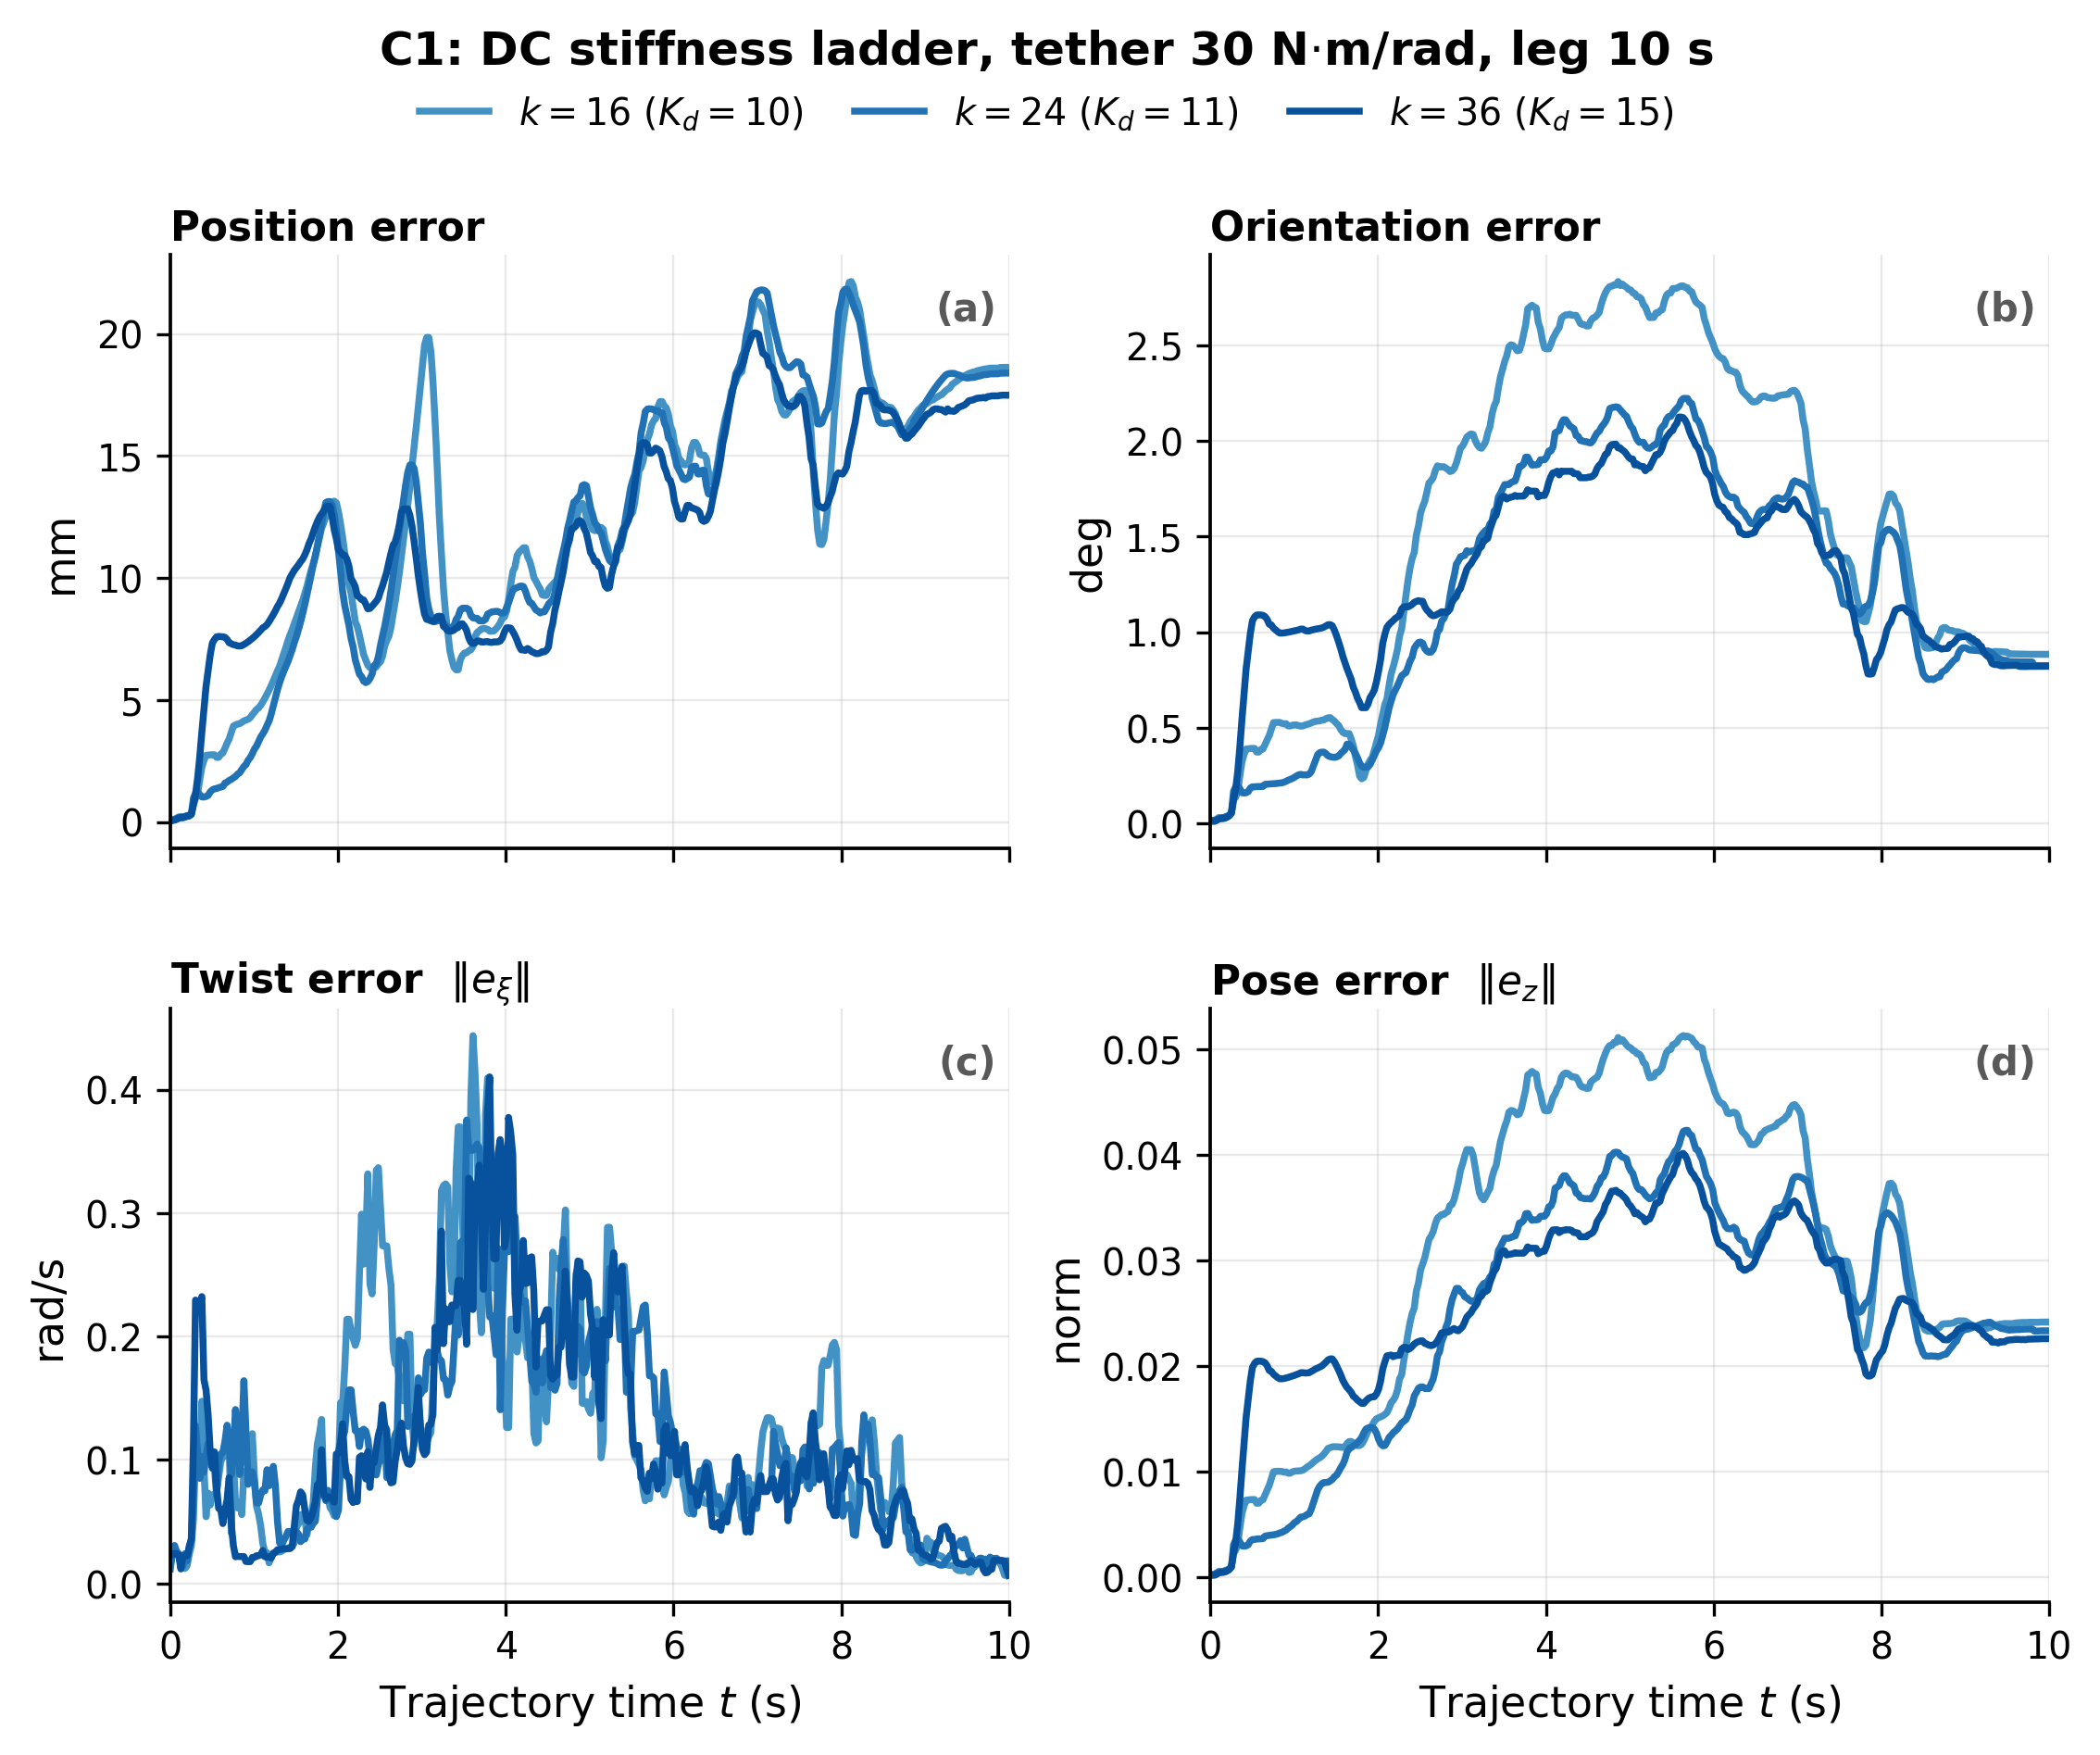
\includegraphics[width=0.44\textwidth]{figures/hw_ts_ladder_C1_tether30_d10.png}\hfill
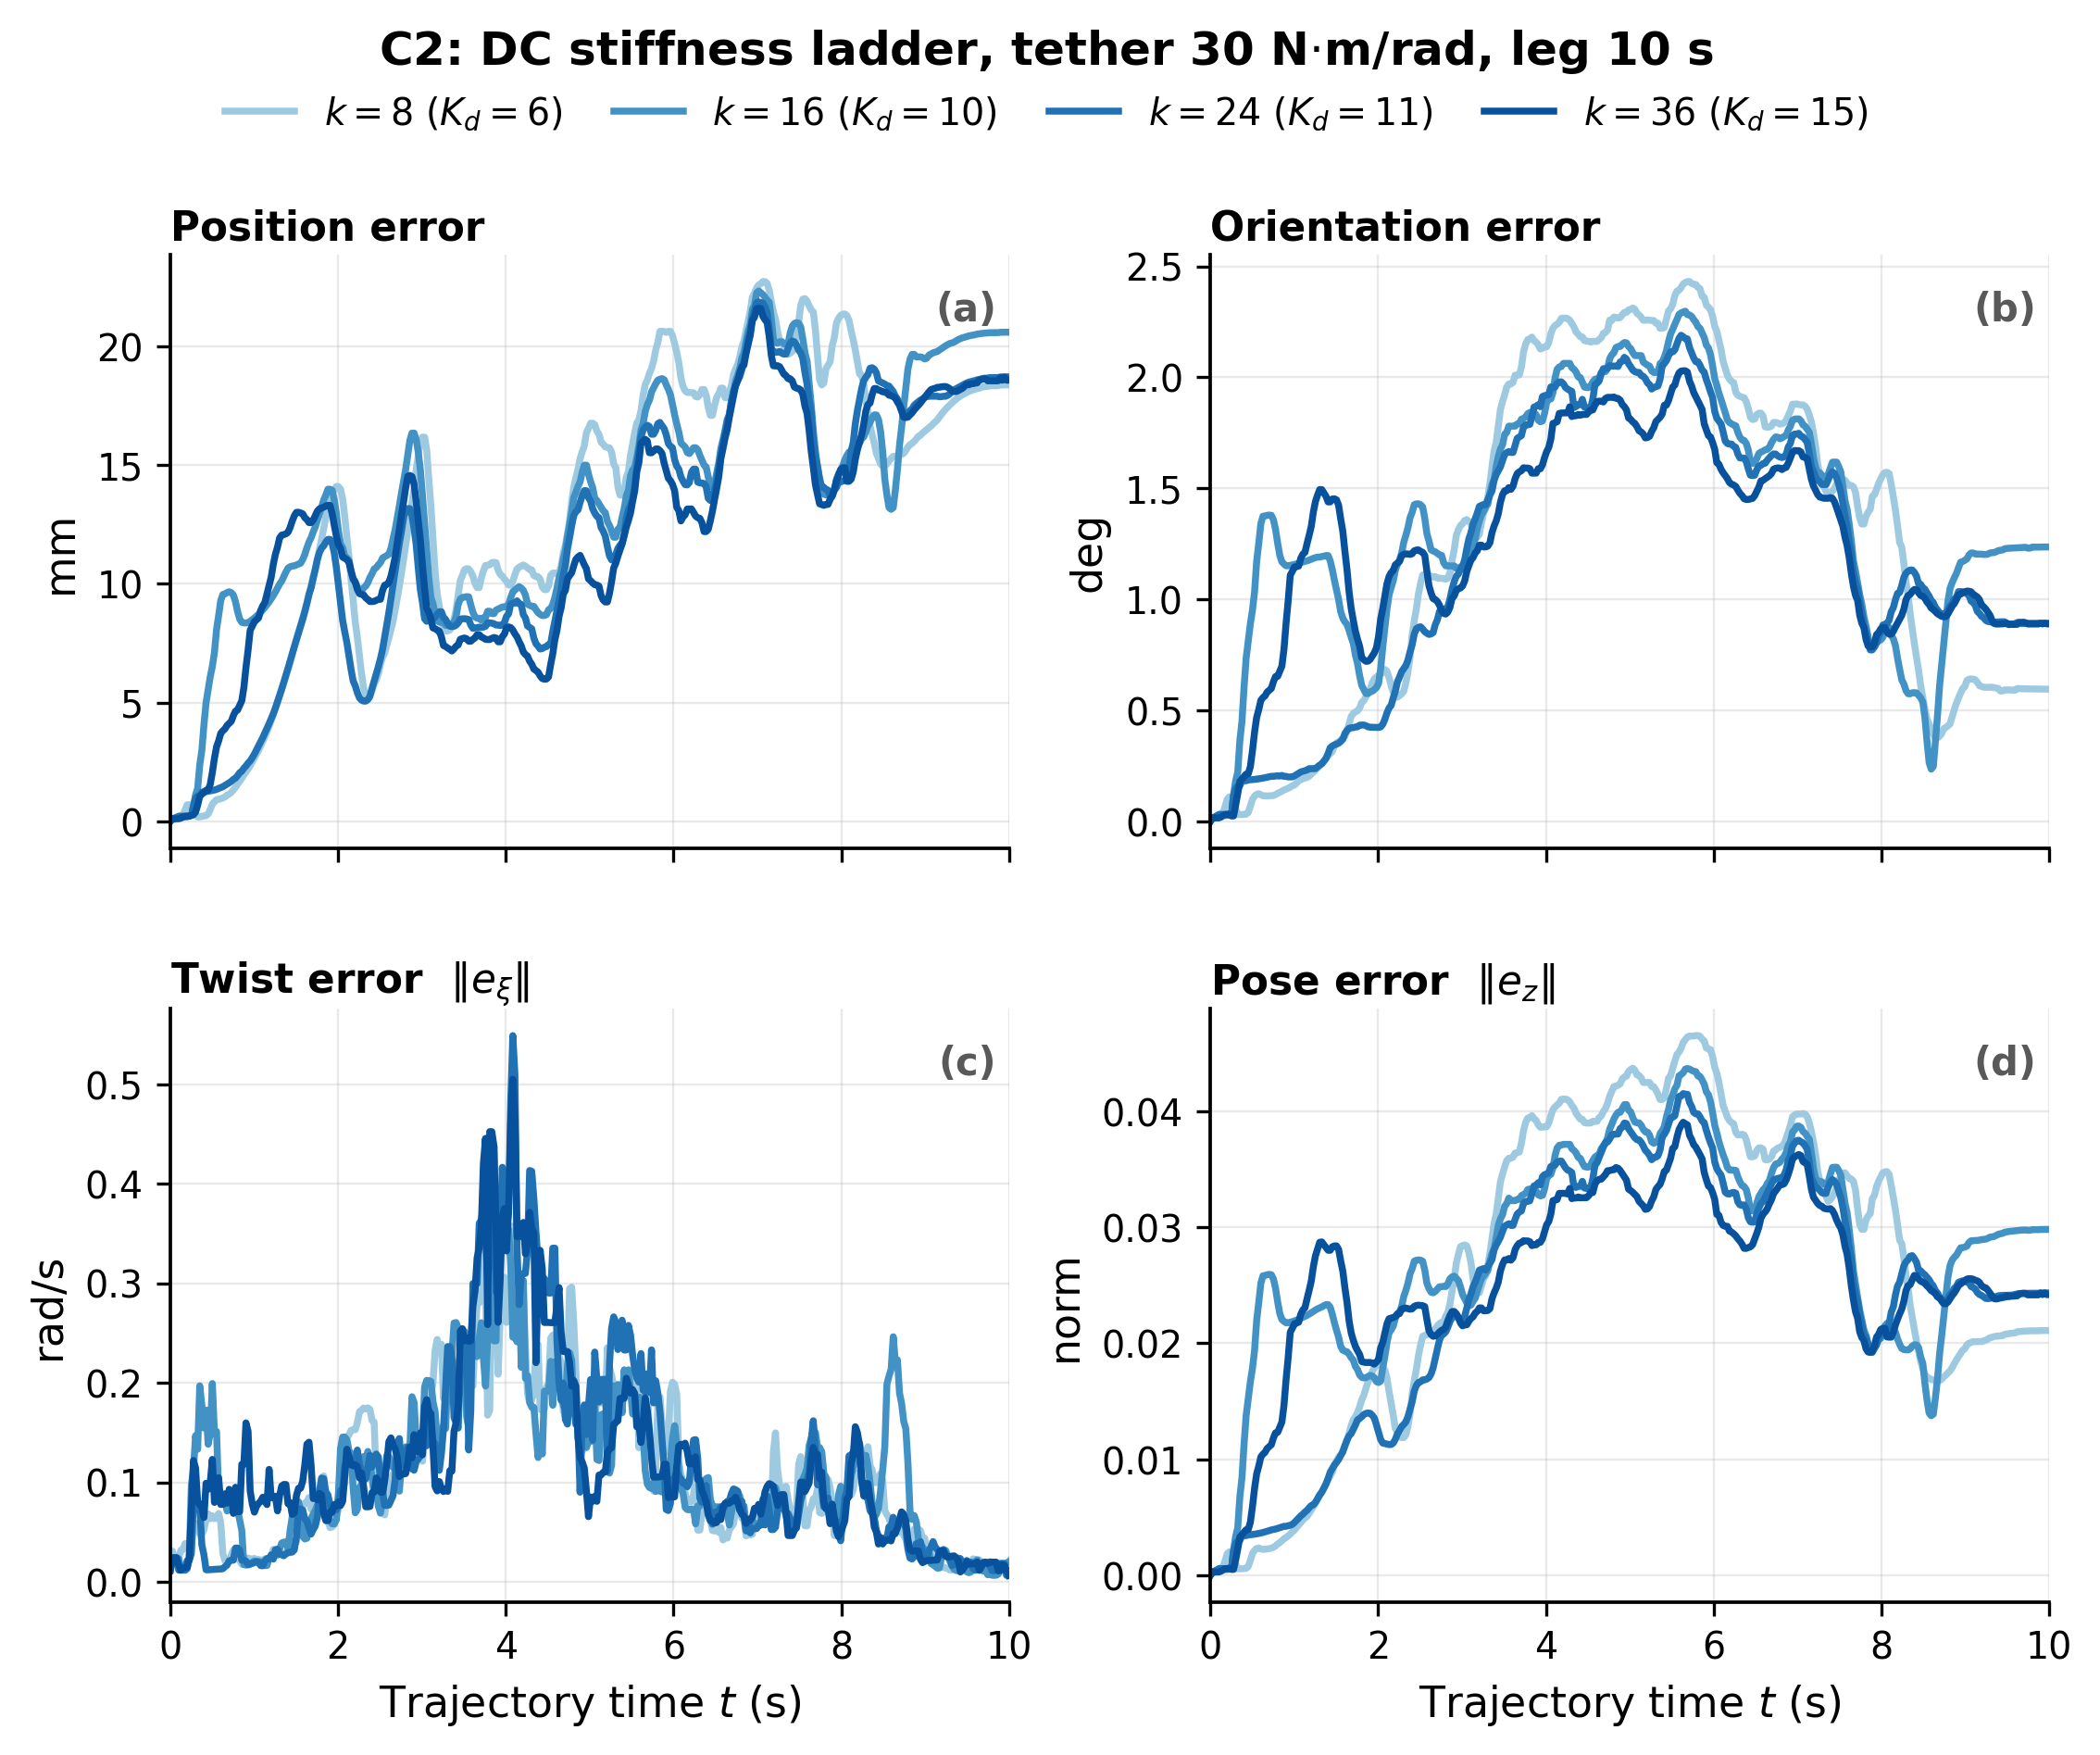
\includegraphics[width=0.44\textwidth]{figures/hw_ts_ladder_C2_tether30_d10.png}\\
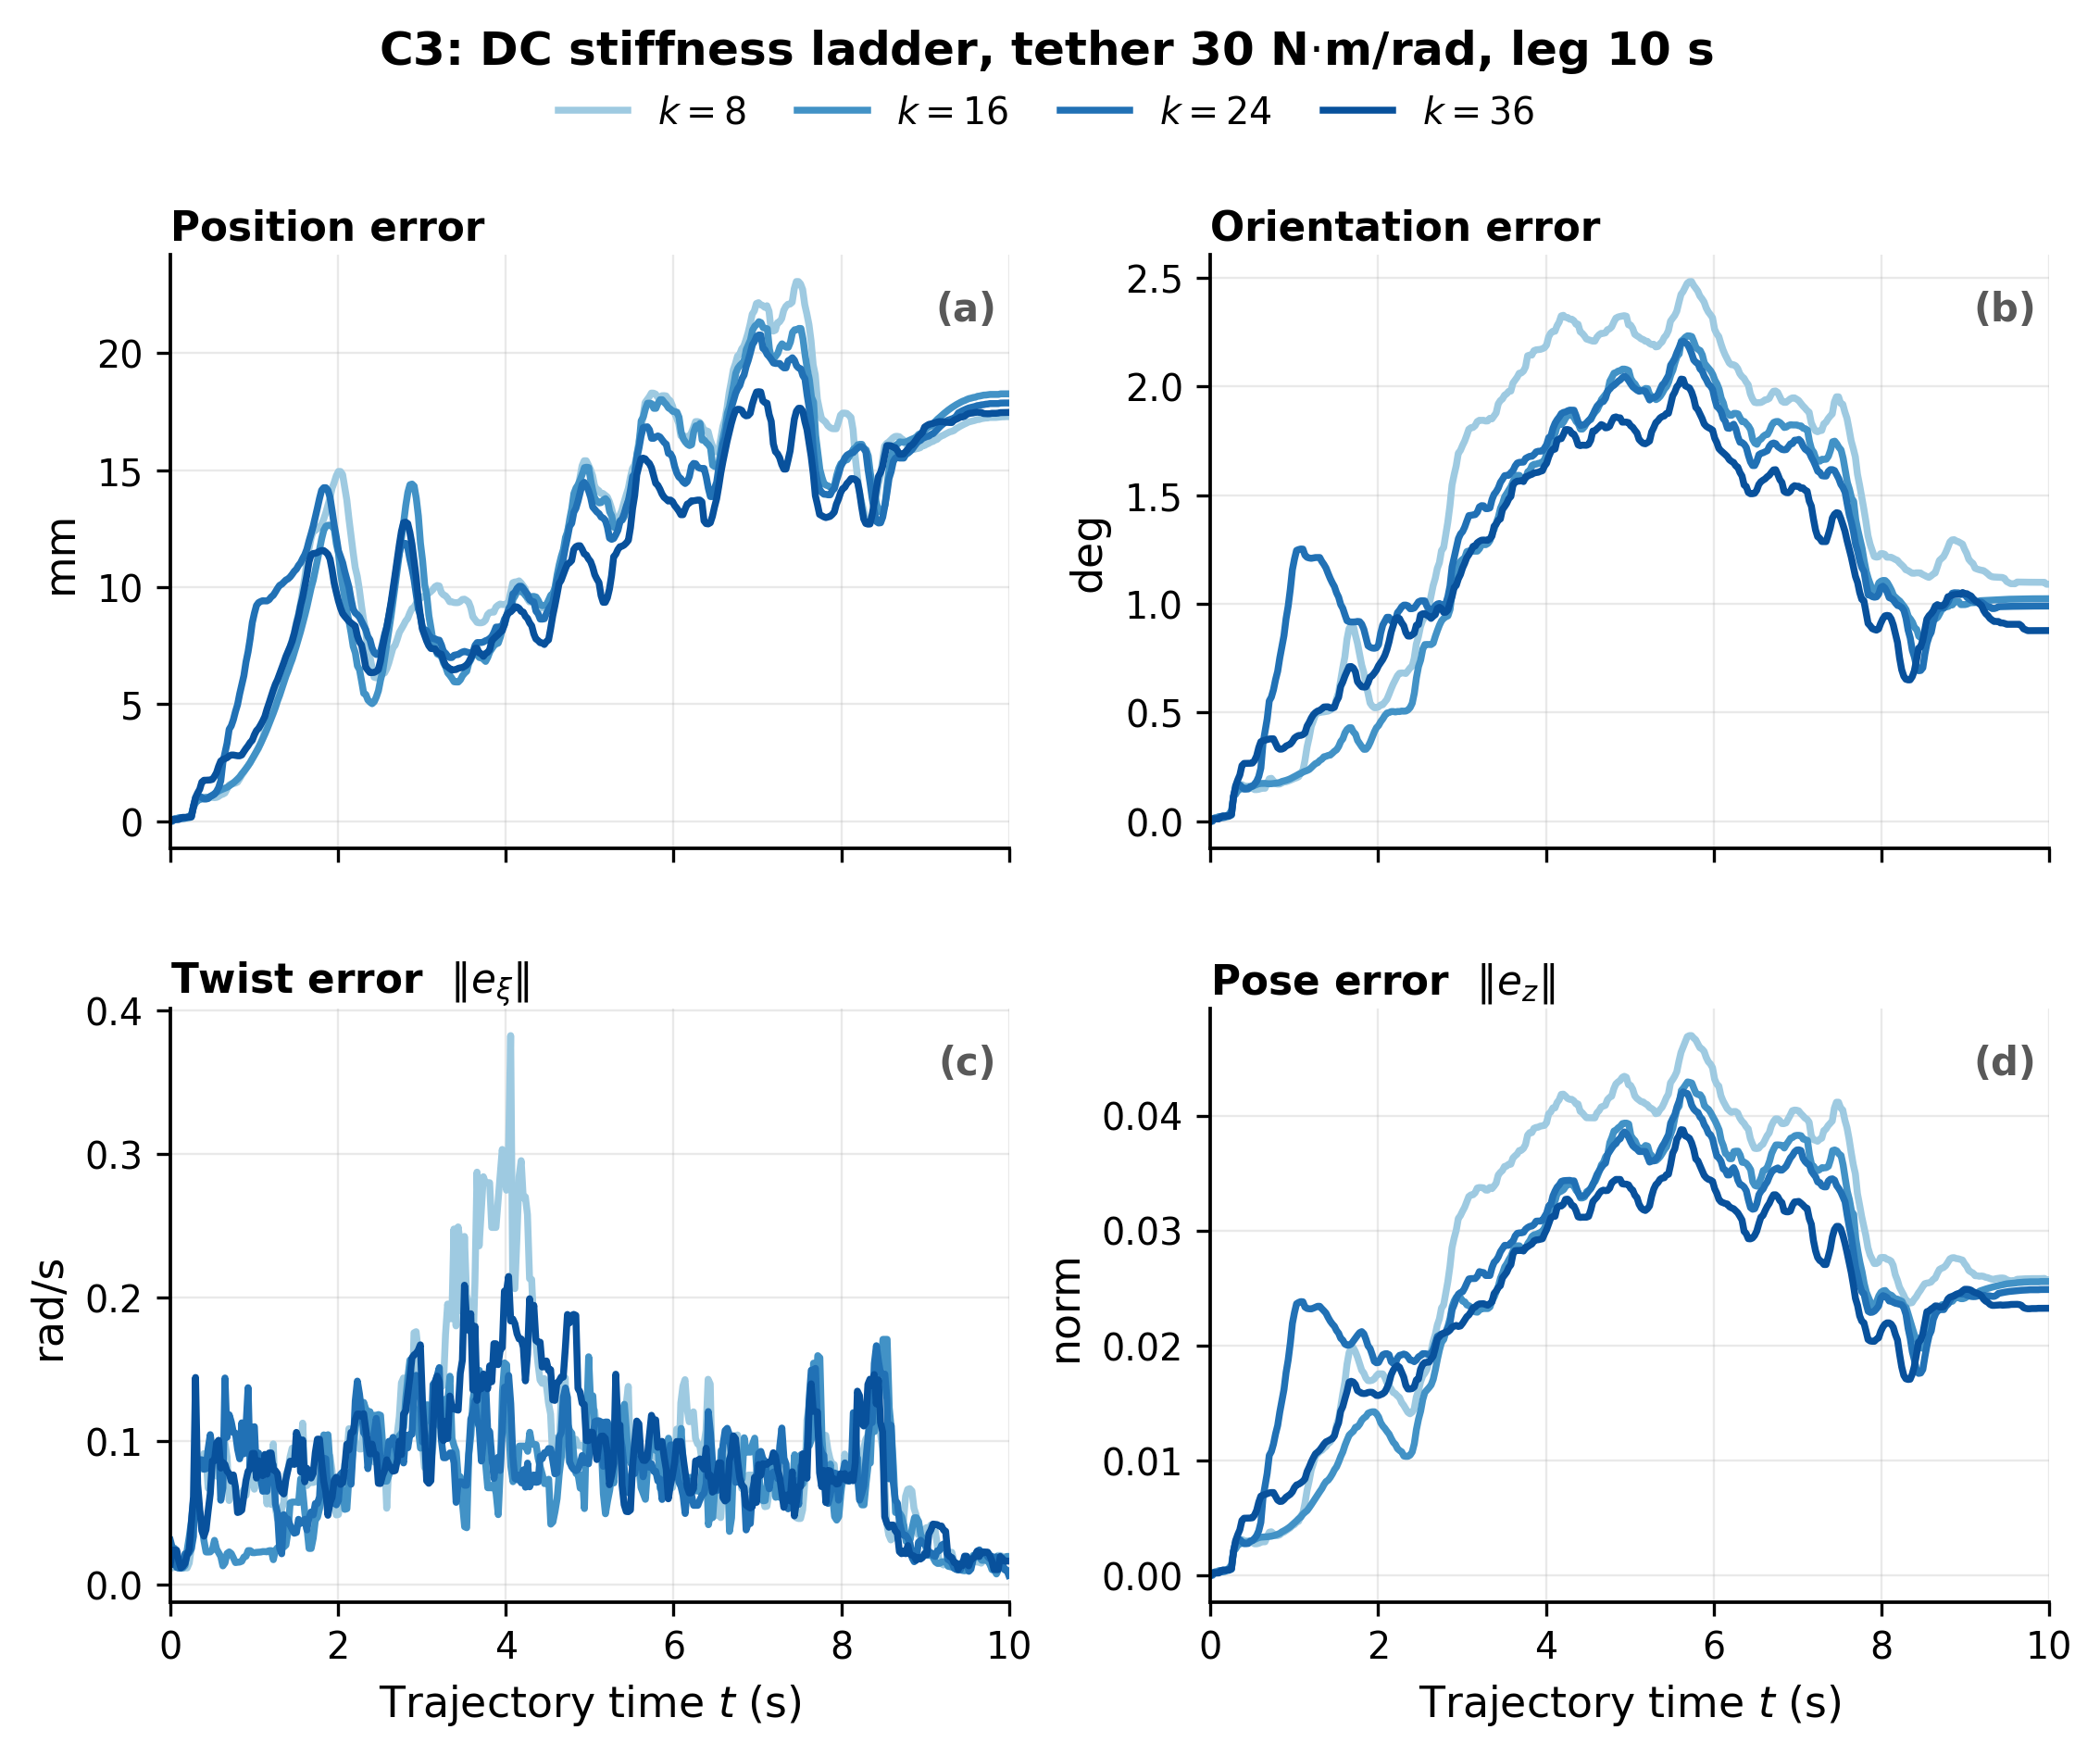
\includegraphics[width=0.44\textwidth]{figures/hw_ts_ladder_C3_tether30_d10.png}\hfill
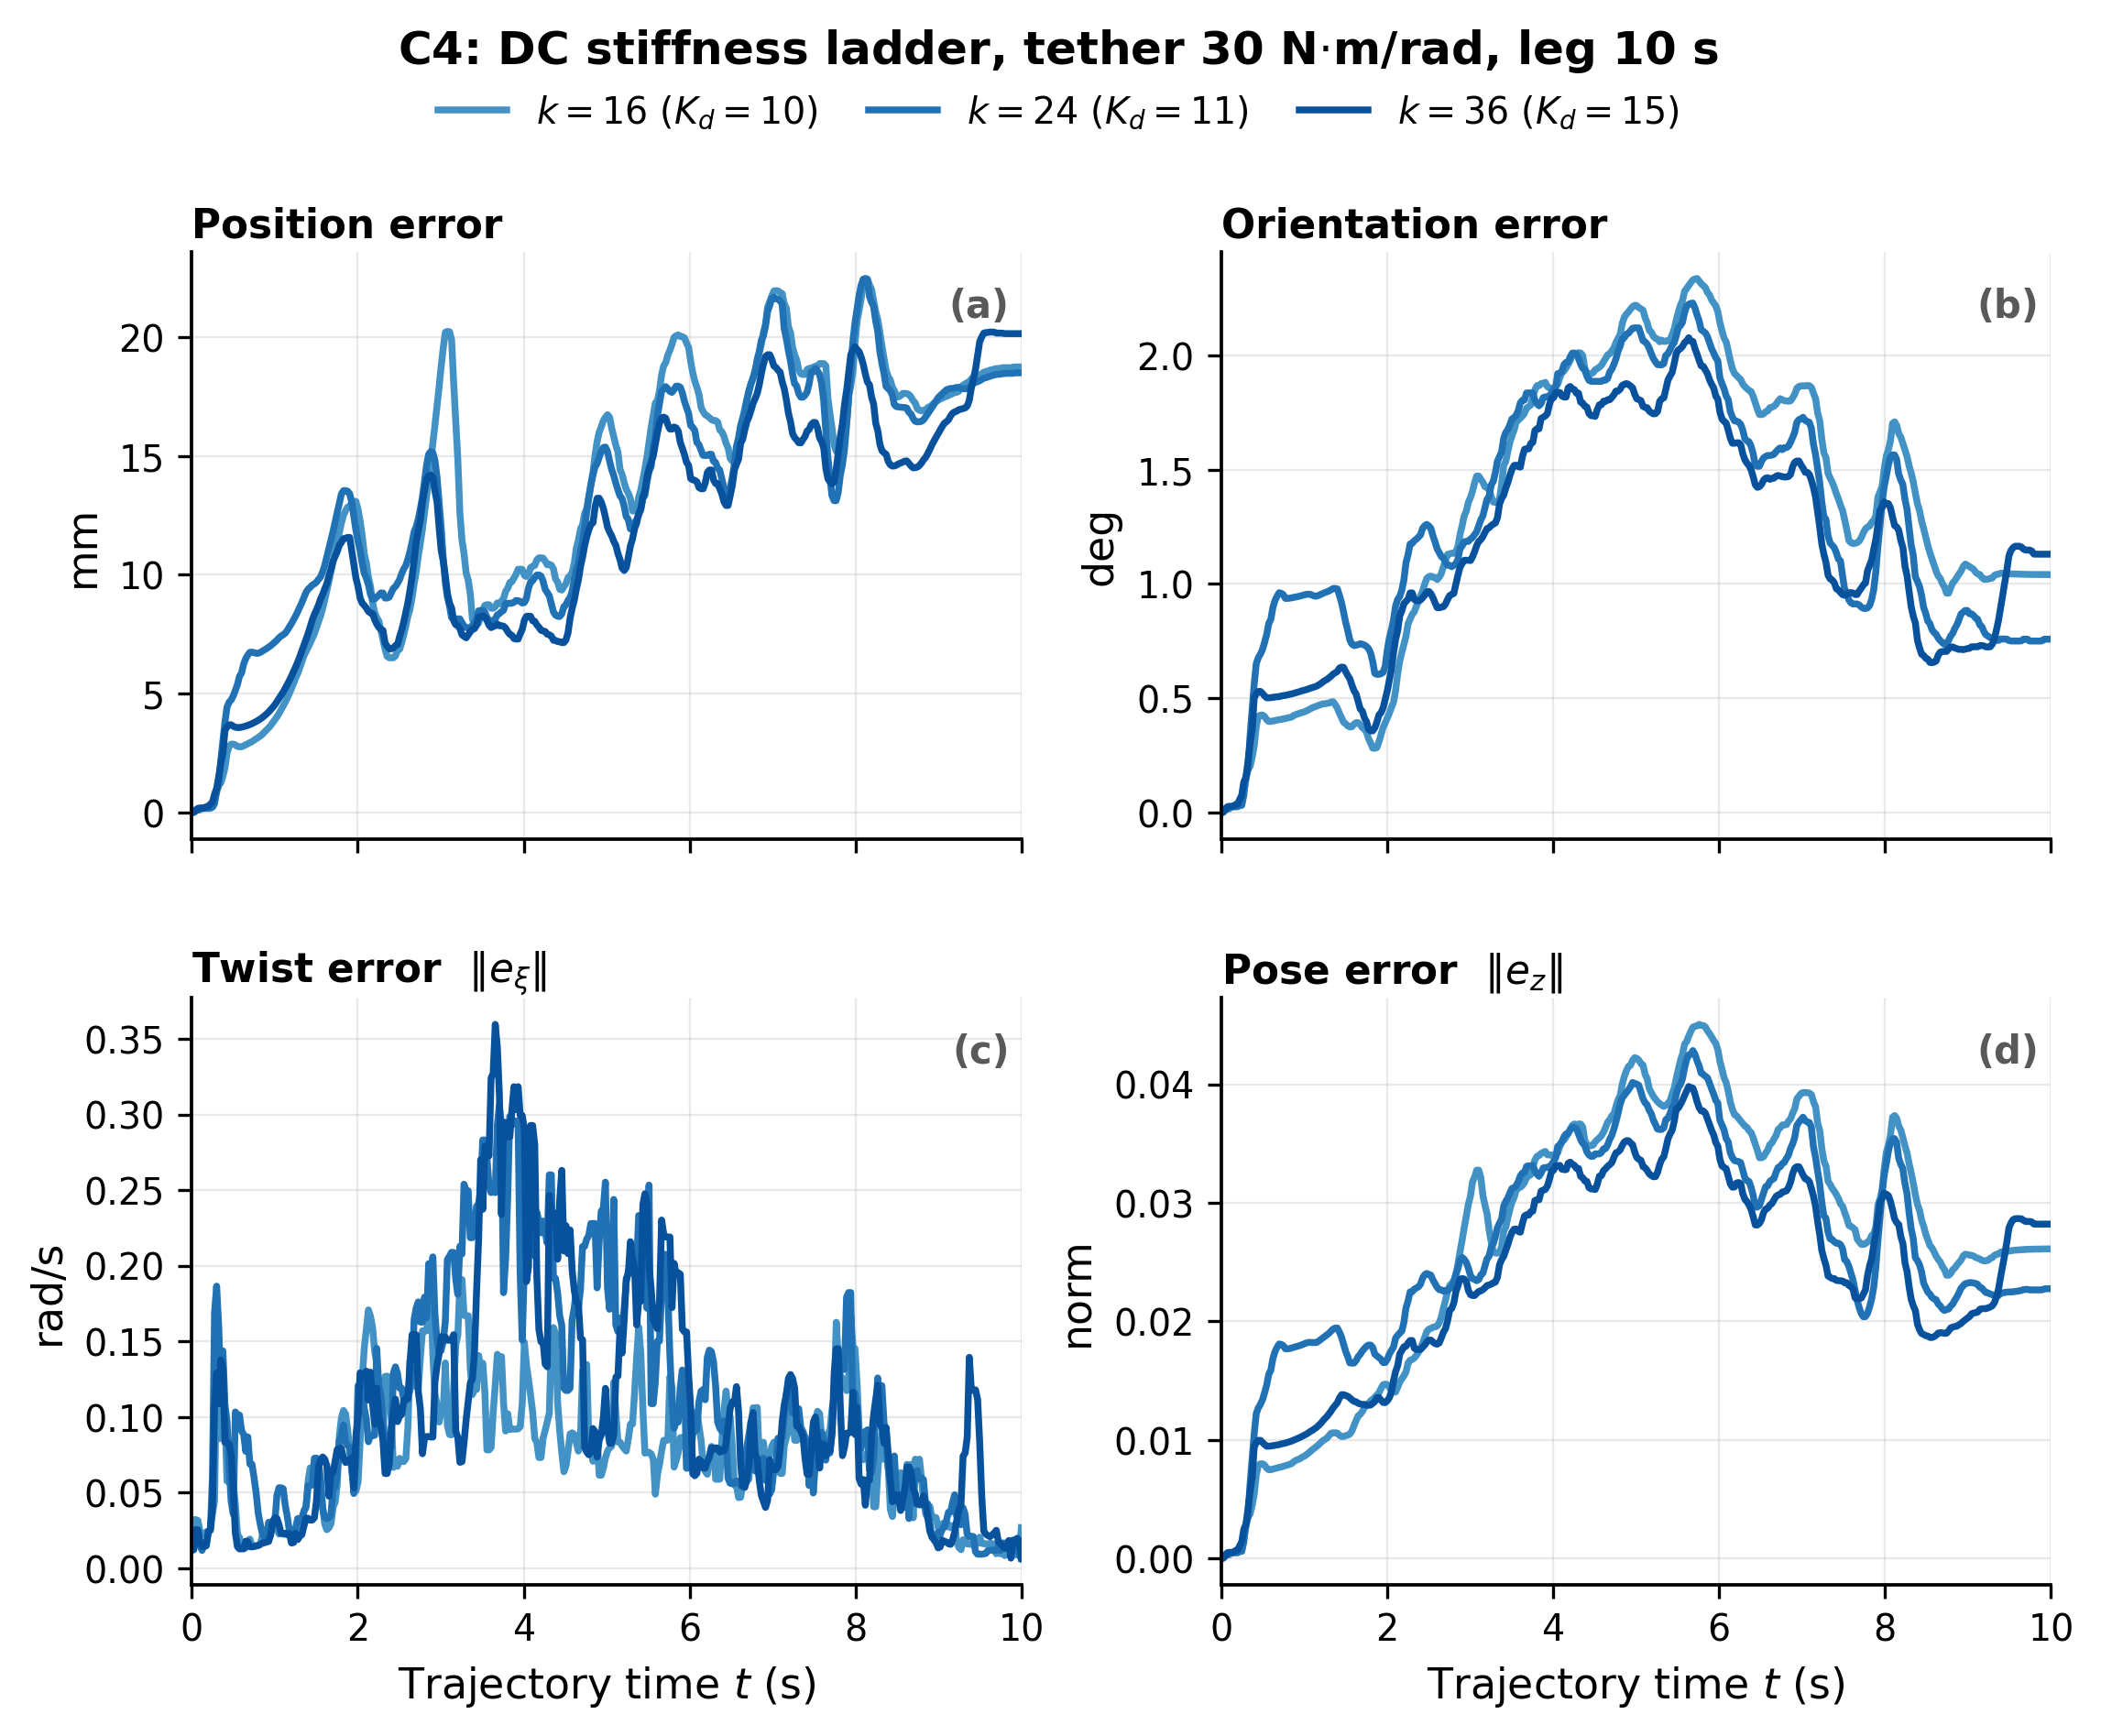
\includegraphics[width=0.44\textwidth]{figures/hw_ts_ladder_C4_tether30_d10.png}
\caption{Gain ladder per law (tether $30\,\mathrm{N\,m/rad}$, the tiers of $k\in\{8,16,24,36\}$ available to each law, single runs of the $10\,\mathrm{s}$ nominal trajectory, aligned on traj\_t): the orientation and twist transients decrease monotonically with $k$ and the position error mildly so, in the direction of tightening $\gamma^{*}$ (Theorem~3(c$'$)).}
\label{fig:hw-ladder}
\end{figure}

\begin{figure}[!tb]
\centering
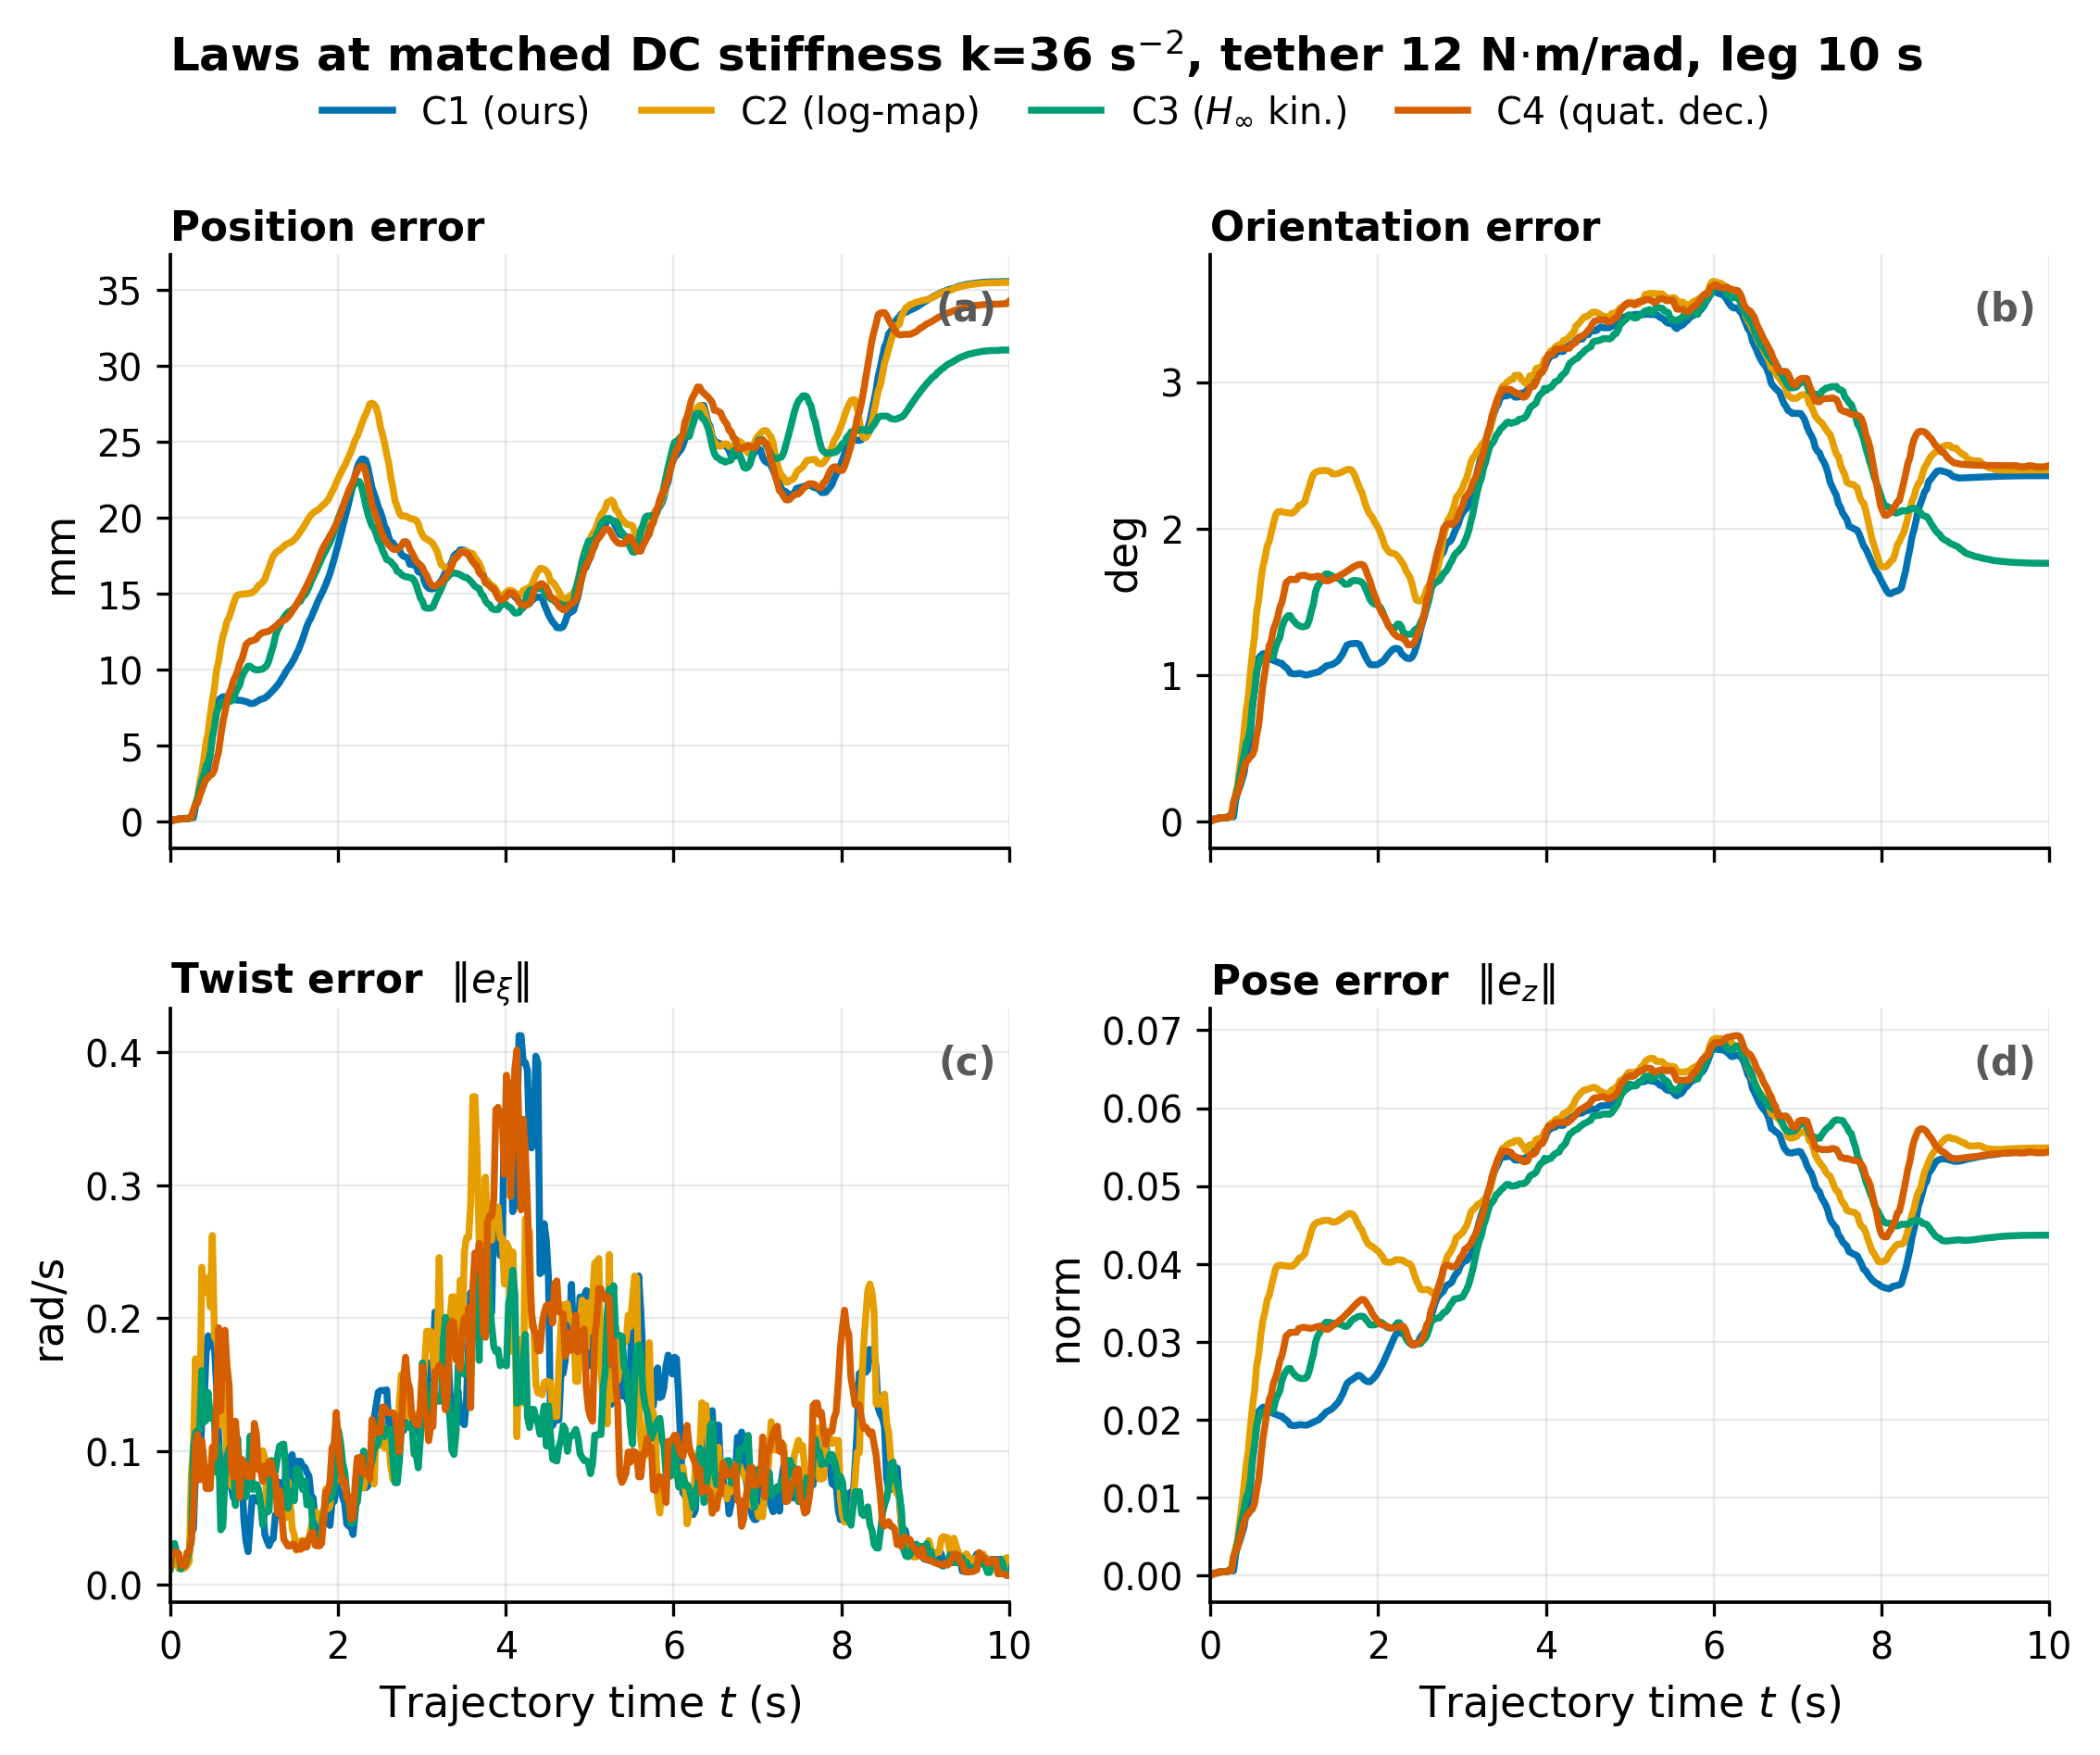
\includegraphics[width=0.49\textwidth]{figures/hw_ts_laws_k36_tether12_d10.png}\hfill
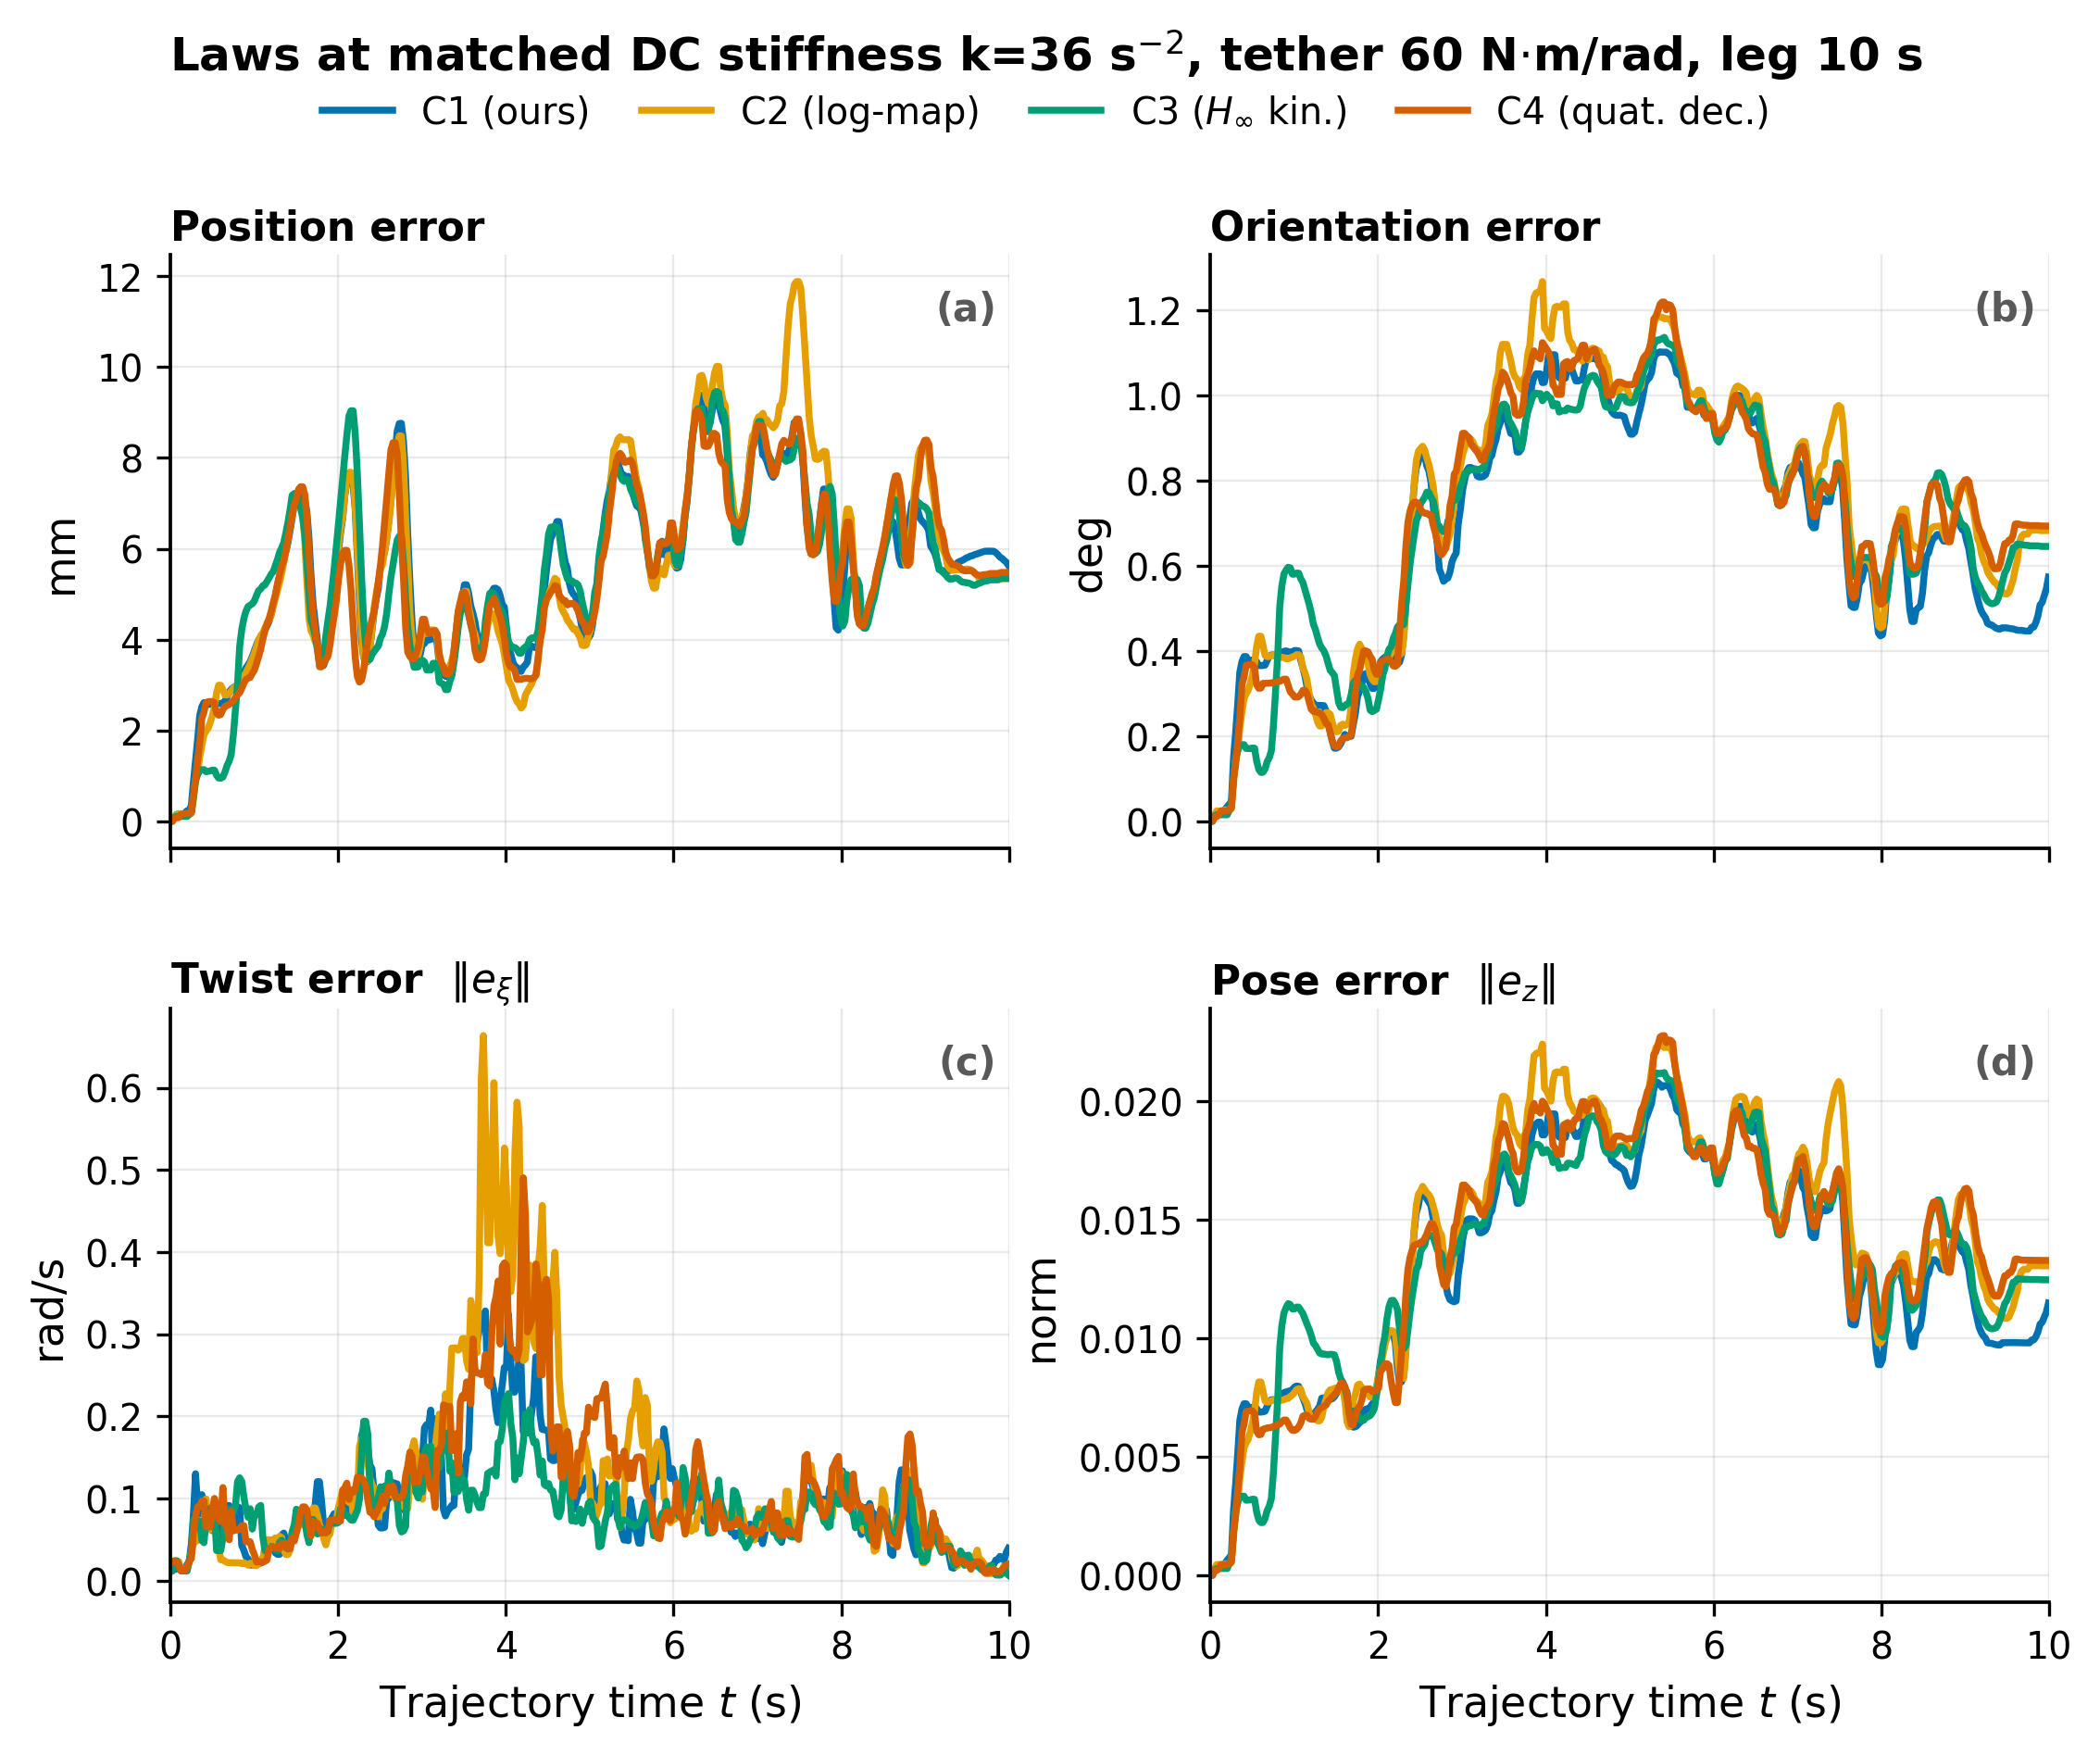
\includegraphics[width=0.49\textwidth]{figures/hw_ts_laws_k36_tether60_d10.png}
\caption{Tether sweep with four laws ($k{=}36$): left, $K_{\mathrm{tr}}{=}12\,\mathrm{N\,m/rad}$ (friction-balance dominated, steady residual $\approx30\,\mathrm{mm}$); right, $K_{\mathrm{tr}}{=}60\,\mathrm{N\,m/rad}$ (millimeter level, steady $\approx5.5\,\mathrm{mm}$). The residual varies nearly inversely with the tether stiffness while the four laws remain on top of each other.}
\label{fig:hw-laws-tether}
\end{figure}

\begin{figure}[!tb]
\centering
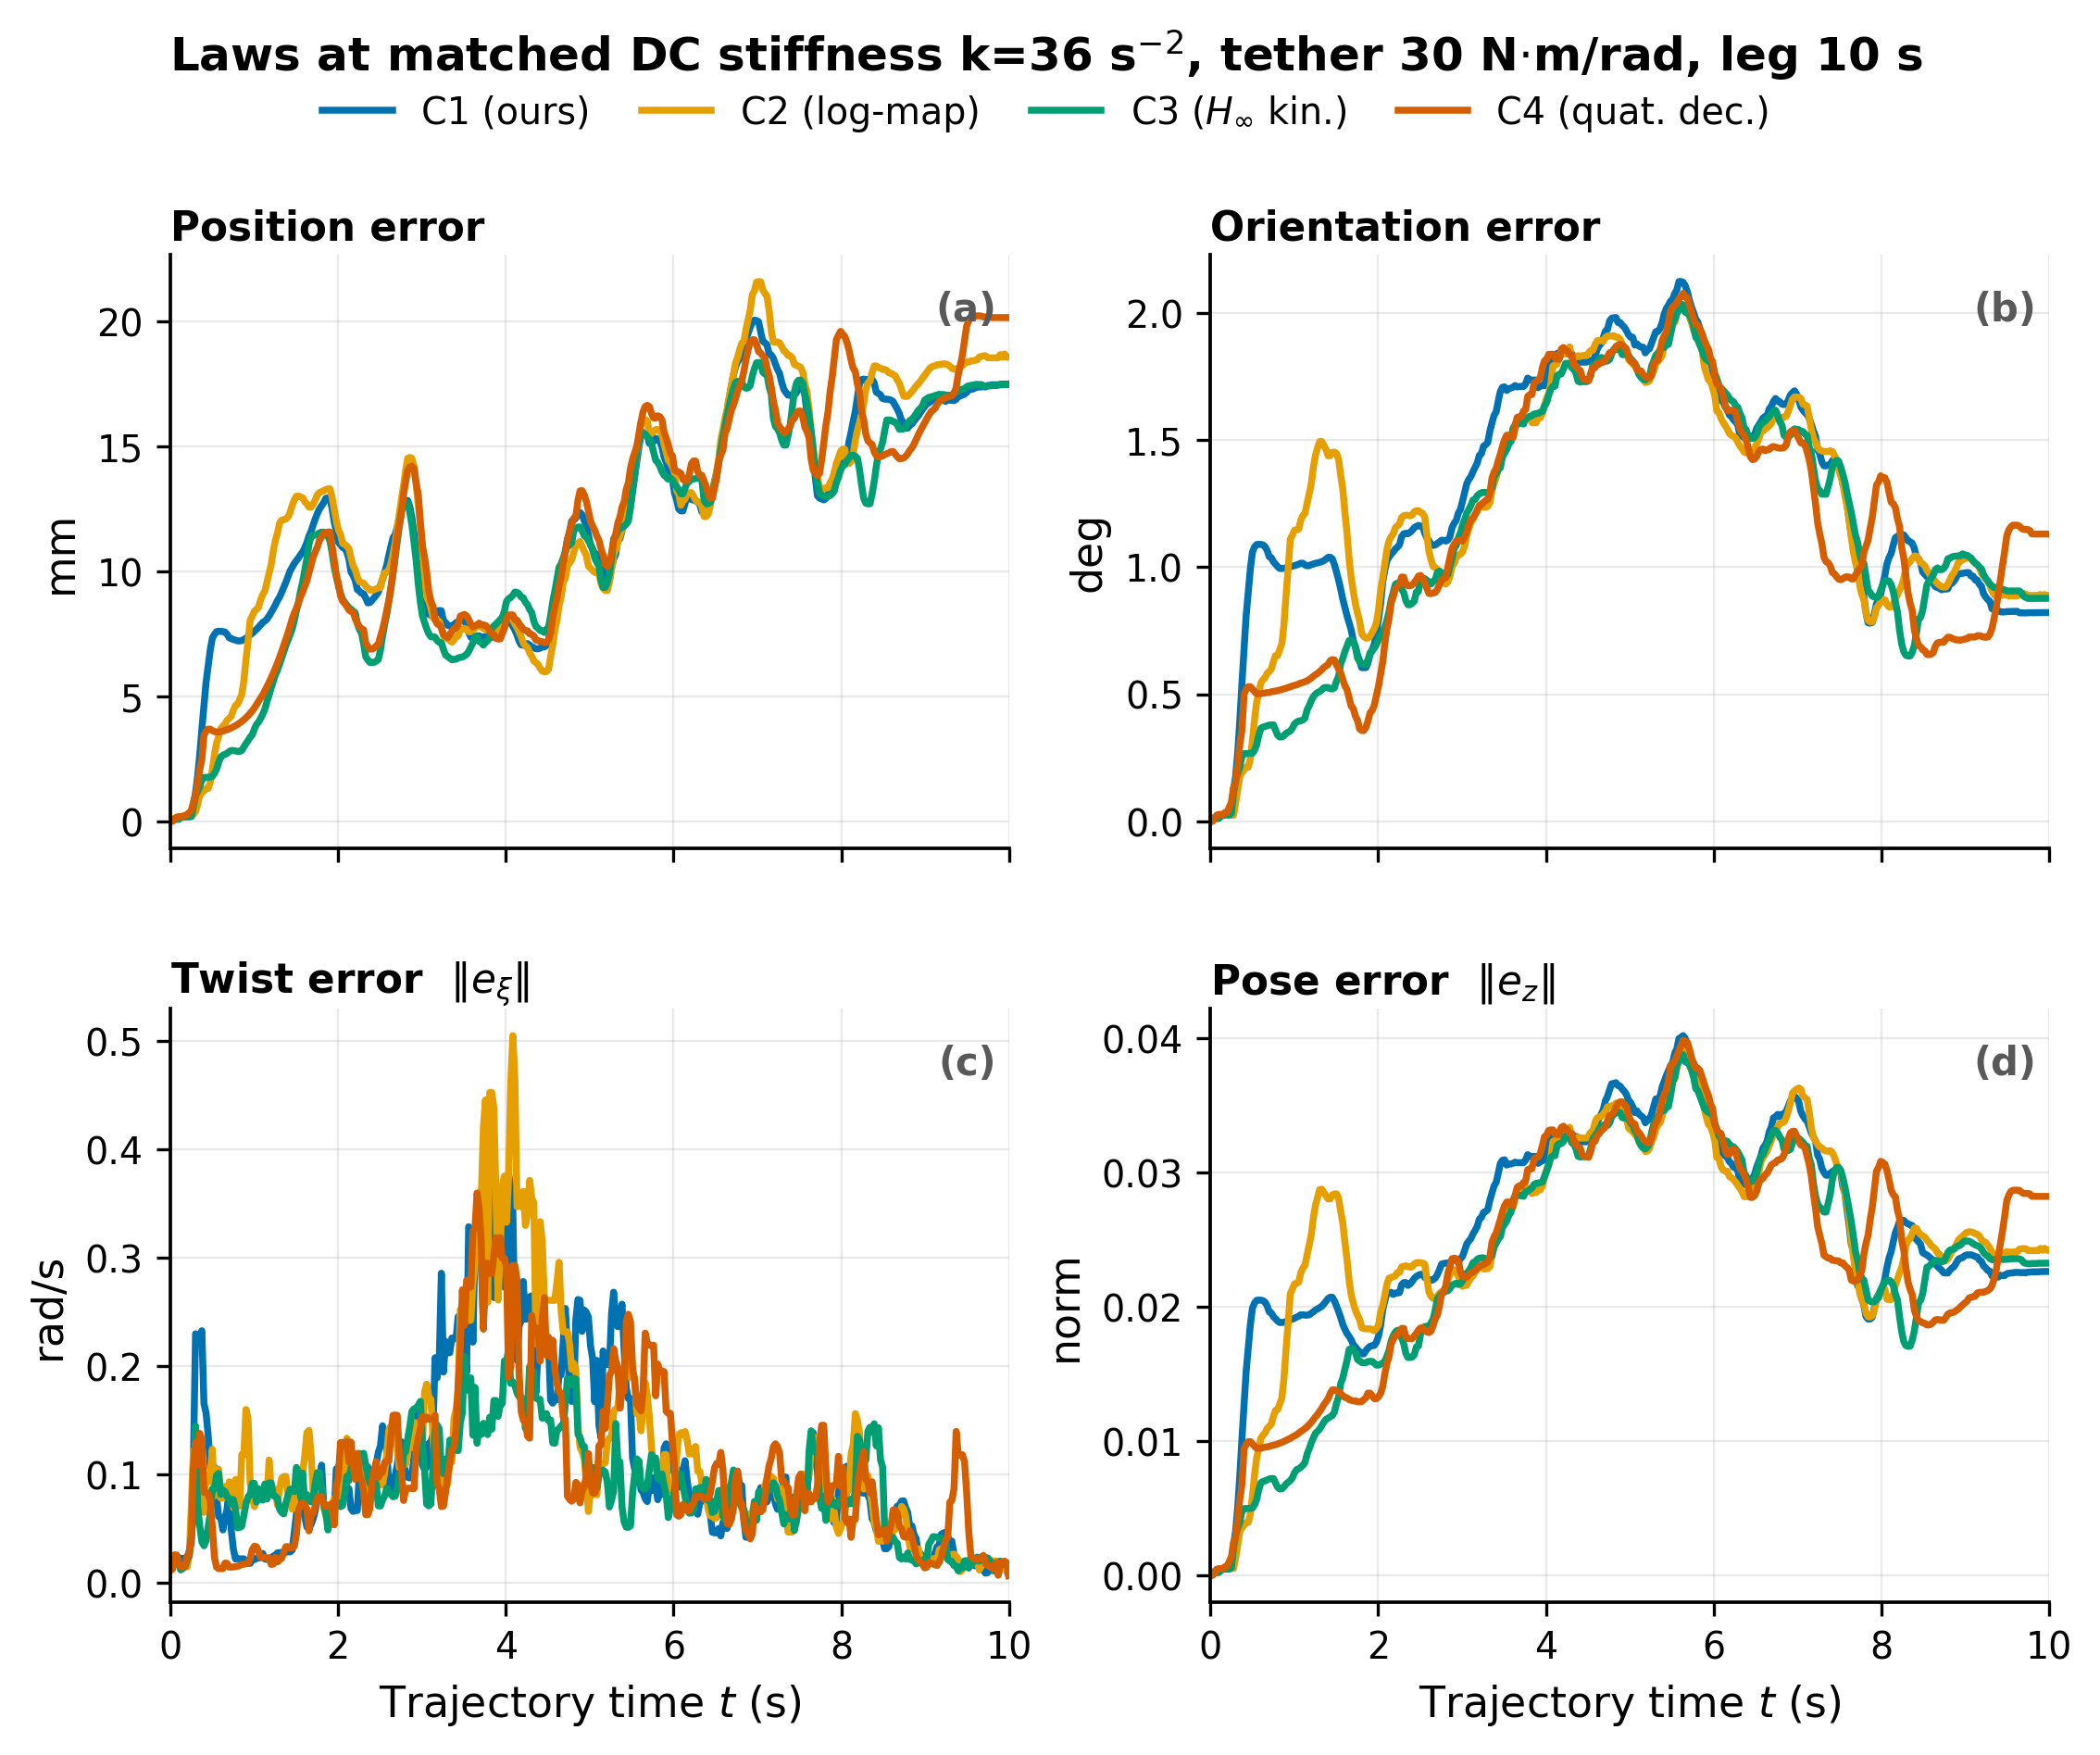
\includegraphics[width=0.78\textwidth]{figures/hw_ts_laws_k36_tether30_d10.png}
\caption{Four laws at equal budget ($k{=}36$, tether $30\,\mathrm{N\,m/rad}$, single runs, $10\,\mathrm{s}$ nominal trajectory): (a) position error; (b) orientation error; (c) twist error $\|e_\xi\|$; (d) pose error $\|e_z\|$. The four curves coincide in all channels, a hardware confirmation of the equal-information-set equivalence; the contribution of C1 lies in the certificate (Table~\ref{tab:hw-gains}), not in accuracy.}
\label{fig:hw-laws-tether30}
\end{figure}
